%!TEX root = ../konzept.tex

\section{Kommunikationsabläufe und Interaktionen}

TODO Alternativen genauer betrachten

Zur Festlegung der Systemarchitektur werden zunächst die Anforderungen anhand eines möglichen Kommunikationsablaufs eines erfolgreichen Interaktionsszenario in einer klassischen Server-Client-Architektur betrachtet (Abb. \ref{fig:kommunikationsablauf}).\\

Ein potentieller Mieter nutzt unsere Smartphone-Anwendung zunächst um seinen eigenen Standort zu ermitteln. Daraufhin sendet er seine Anfrage an unser Hauptsystem, welches das erste \textit{Matching} durchführt.

In einer Datenbank befinden sich Zuordnungen zwischen Vermieter und dem Ort eines Mietobjektes. Auf Basis dieser Datenmenge wird ein Abgleich zwischen angefragtem Ort und vorhandenen Orten durchhgeführt. Bei allen möglichen Treffern wird der zugehörige Nutzer herausgefiltert.

Zu den relevanten Daten eines Nutzers gehört unter anderem eine Identifikationsnummer, unter welcher das Smartphone des Nutzers ansprechbar ist.
Dadurch werden die nun gefilterten Vermieter angesprochen und bekommen ein Ereignis zugesendet.

Das Ereignis beinhaltet die relevanten Daten der Anfrage durch den Mieter. Sobald das Ereignis das Ziel erreicht hat, wird auf dem Endgerät des Vermieters das zweite \textit{Matching} durchgeführt, denn wie in der Martkanalyse bereits identifiziert wurde, werden direkte Personen- und Objektdaten auf den Endgeräten der Nutzer gespeichert.

Das zweite \textit{Matching} vergleicht das gesendete Profil mit dem auf dem Gerät gespeicherten Profil. Ein Algorithmus berechnet dabei einen Quotienten, welcher den Grad der Übereinstimmung widerspiegelt. Übersteiget dieser Quotient einen Wert X, wird der Vermieter über die Anfrage visuell über die Anfrage benachrichtigt, auf welche dieses reagieren muss.
Der Vermieter kann die Anfrage bestätigen oder ignorieren. Bei einer Bestätigung wird der Mieter über die Bestätigung informiert und kann die Daten des potentiellen Mietobjektes einsehen, sowie weiteren Kontakt zu dem Vermieter aufnehmen.

\begin{figure}[H]
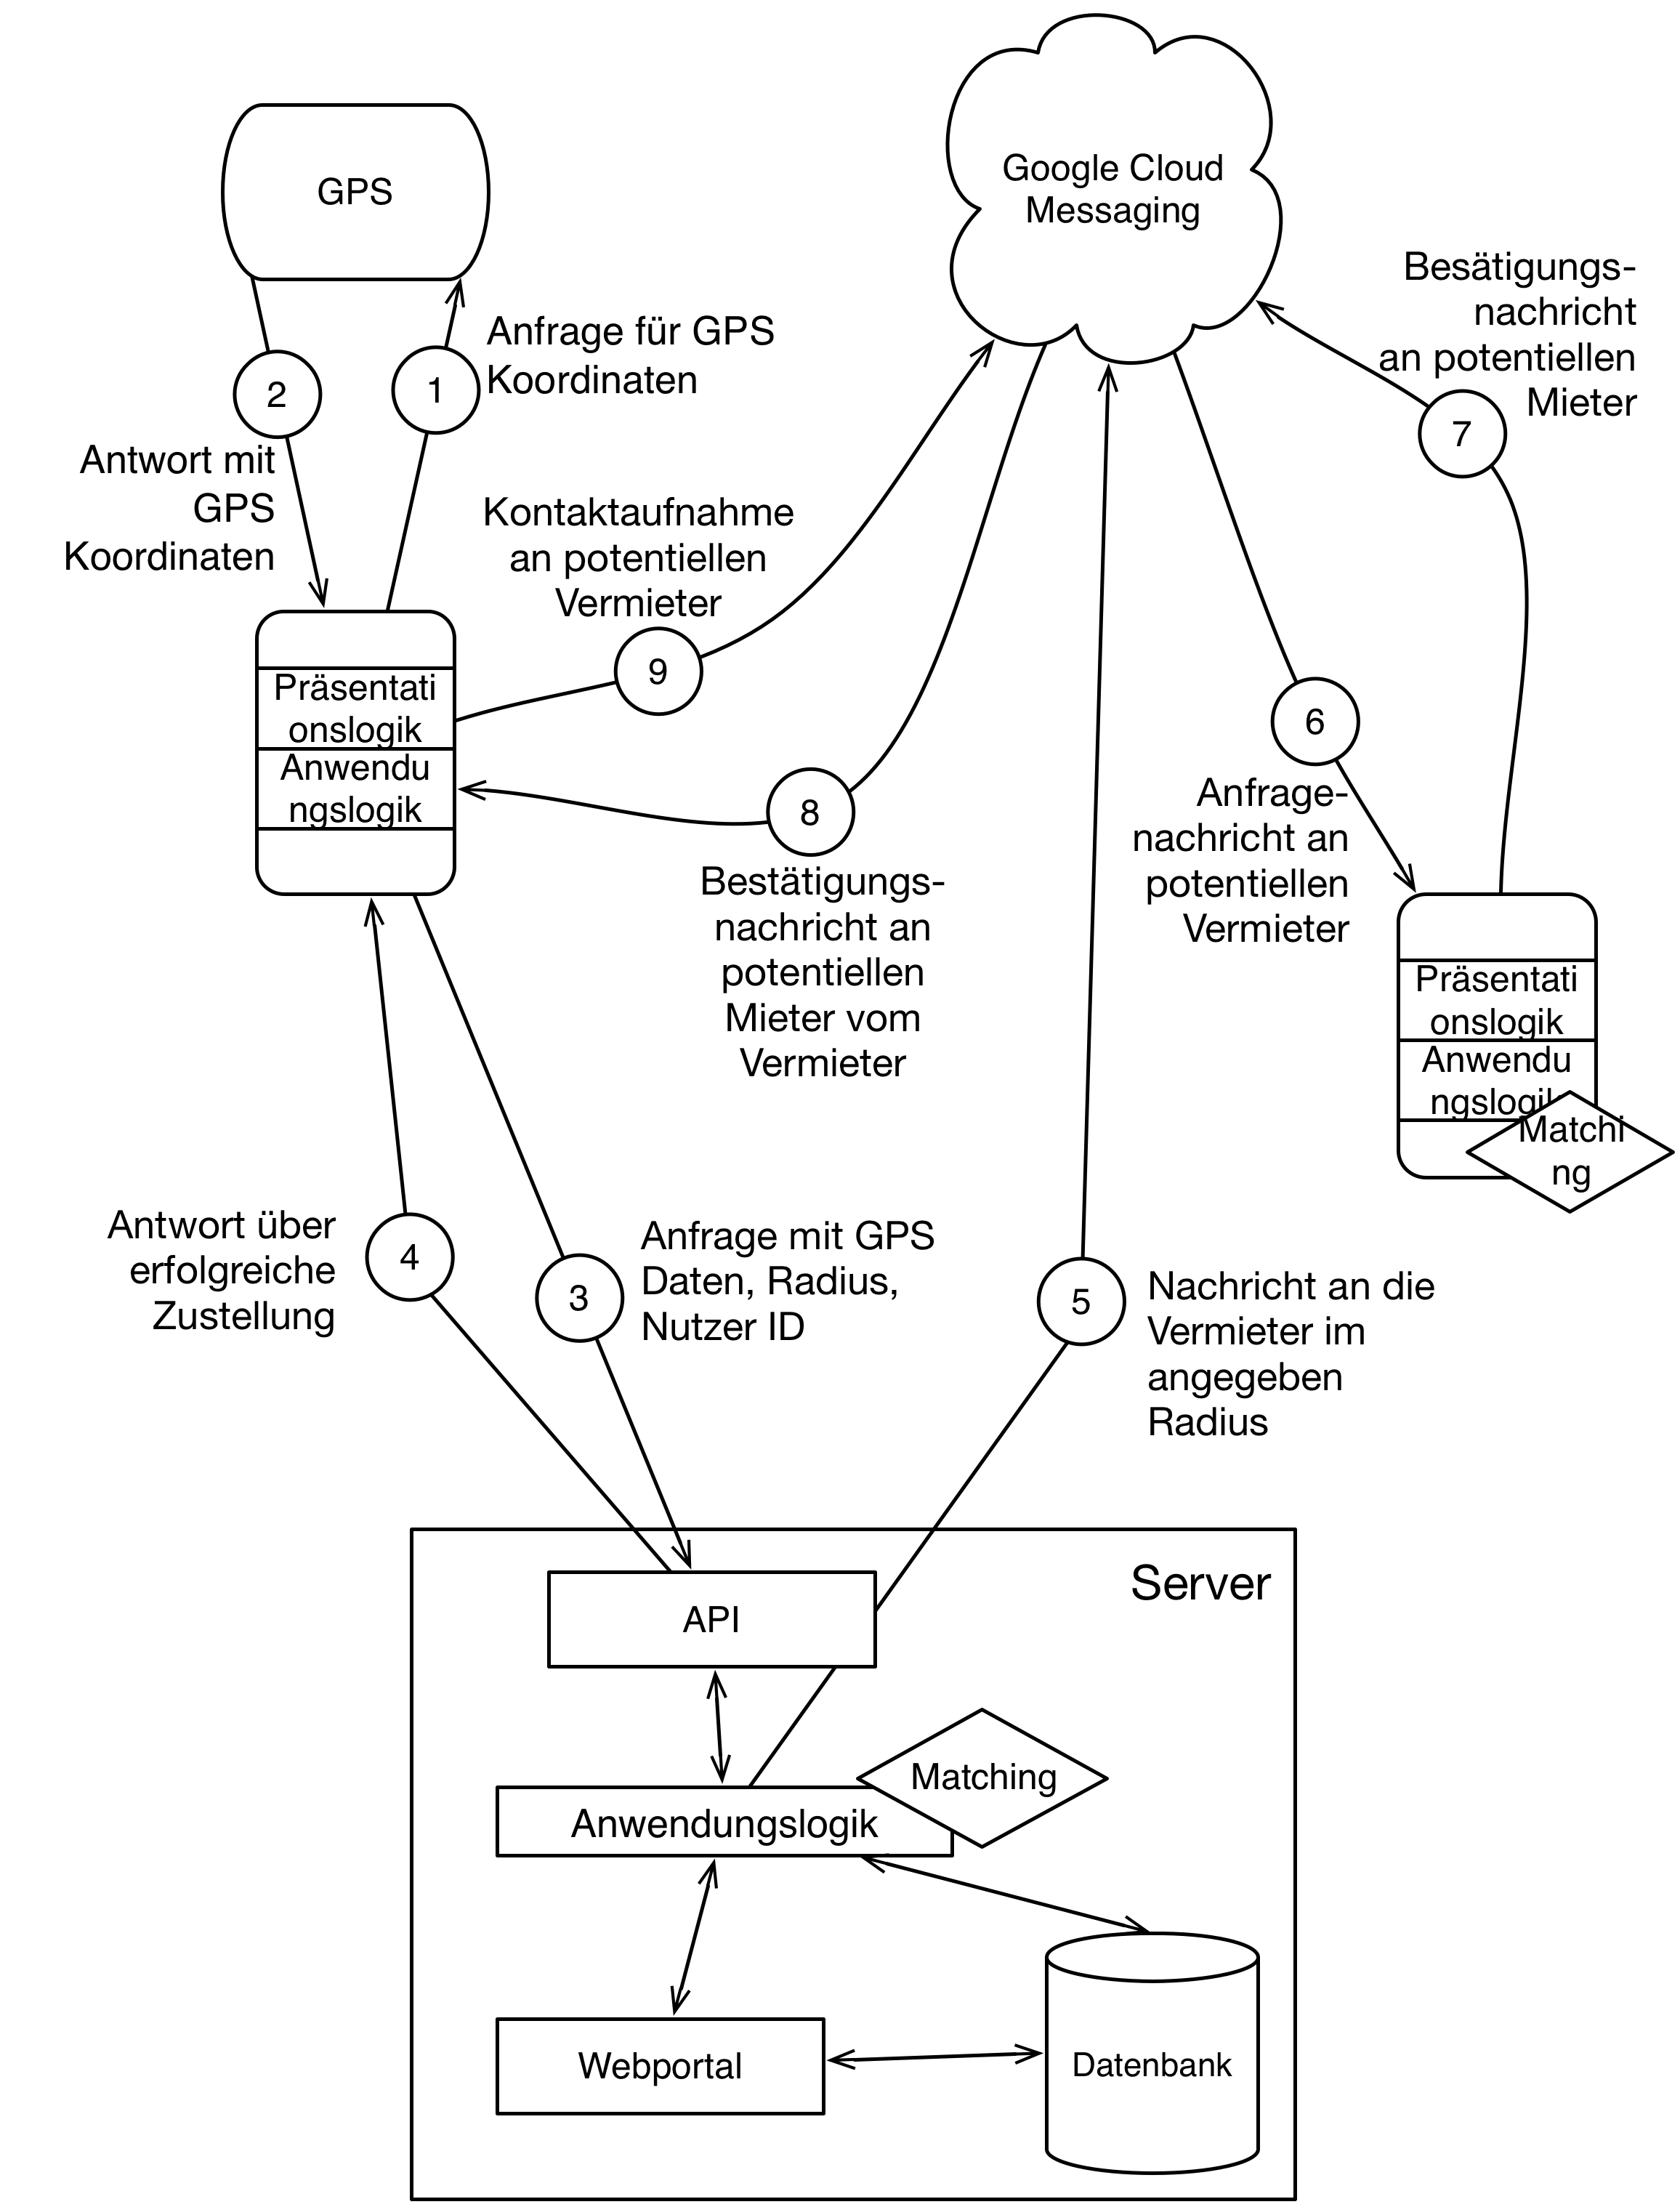
\includegraphics[width=.9\textwidth]{./images/kommunikationsablauf.png}
\caption{Kommunikationsablauf eines erfolgreichen Interaktionsszenario }
\label{fig:kommunikationsablauf}
\end{figure}

Auf Basis dieses Kommunikationsablaufs kann nun auf die einzelnen Komponenten der Systemarchitektur eingegangen werden.

